\section{Background}
\label{sec:Background}

In this section, we will explain the necessary concepts on which our approach builds. First, in \cref{sec:ViewBasedDevelopment}, we will explain different solution strategies to view-based development, as well as a short introduction to the development process in view-based environments. \Cref{sec:ViewGeneration} will then explain how views are generated and the impact of different view generation languages on our approach to \metamodel \viewtype co-evolution. Finally, in \cref{sec:MetaModelEvolution}, we will provide an explanation on how we break down \metamodel evolution in semantically meaningful steps and how these steps can be detected a posteriori.

% \MA{Does it make sense to split the Section into two: (i) Views; (ii) View Generation (or something similar)}

\subsection{View-Based Development}
\label{sec:ViewBasedDevelopment}

There is a distinction between \emph{synthetic} and \emph{projective} approaches to view-based modeling \autocite{atkinson_fundamental_2015}.
In synthetic approaches, the system is represented by the union of all views.
For that purpose, changes must be propagate between the views to ensure the system description is consistent.
This is different in projective approaches where, in addition to the views, an underlying model of the system exists, which is the source of all information.
Views in projective approaches are transient, i.e., not persistent, and generated dynamically from the underlying model whenever they are required \autocite{atkinson_orthographic_2010}.
With projective views, the user is only allowed to interact with the system through the views, while the underlying model is usually hidden.
In particular, when a user wants to make changes to the system, the changes need to be applied to (editable) views first and are then propagated to the underlying model.
The relationship between views, \viewtypes, models and \metamodels in projective approaches is shown in \cref{fig:view_concept}.
The \cite{ISO42010} standard also contains a definition of the \emph{view} concept, as well as of synthetic and projective approaches, but in a broader sense for software architecture and software architecture description languages.

\begin{figure}
    % TODO recreate figure (with \metamodel and \viewtype)
    \begin{center}
        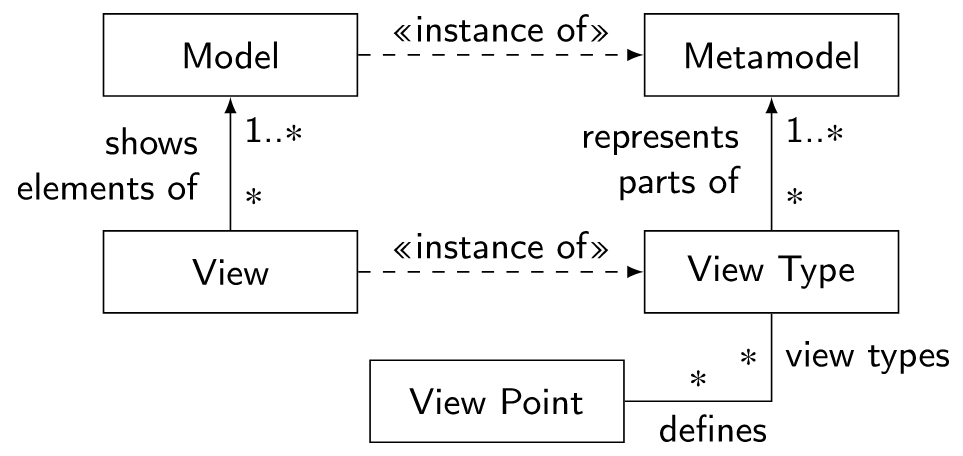
\includegraphics[width=\linewidth]{images/ViewTypeTerminology.png}
    \end{center}

    \caption{Visualization of the view terminology for projective approaches as defined by \textcite{burger_flexible_2014} and \textcite{klare_enabling_2021}.}
    \label{fig:view_concept}
\end{figure}

For projective view-based environments there are different ways of constructing the (single) underlying model (SUM).
\Textcite{atkinson_fundamental_2015} differentiate between \emph{essential} and \emph{pragmatic} SUMs.
With an essential SUM there is a single model, which contains the complete system description and is free of any internal redundancies.
For the synchronization between the views, this is the easiest solution, because the views are simply required to write the changes back to the SUM.
Subsequently generated views are then automatically consistent.
An example of an approach employing an essential SUM is OSM by \textcite{atkinson_orthographic_2010}.
In contrast to a single redundancy-free model, there are also pragmatic approaches where the underlying model consists of multiple submodels.
The main benefit of pragmatic approaches is the construction of the underlying model.
While it is difficult to create a single redundancy-free \metamodel, especially for a domain-spanning system, pragmatic SUMs allow the integration of already available \metamodels, e.g., from development tools used in the various domains.
Additional effort is, however, necessary to keep the models consistent.
One framework for constructing pragmatic SUMs, here called virtual SUMs (V-SUMs), is Vitruvius \autocite{klare_enabling_2021}.

\Textcite{atkinson_orthographic_2010} identified two roles when employing a view-based development process.
First, the \emph{methodologist} is responsible for creating the view-based environment.
For this, the methodologist creates or assembles the SUM, which includes specifying the consistency relations between the models, if necessary.
In addition, they define the view types on the system, including rules how changes are propagated back to the underlying model.
The second role, the \emph{developer}, uses the environment created by the methodologist to develop the actual system.
The developer creates views on the system to inspect its properties and performs changes on them, which are then applied to the underlying model.

\subsection{View Generation}
\label{sec:ViewGeneration}

Since the content of projective views is derived from the underlying model, the methodologist must define a \emph{view generation transformation (VGT)} for each view type, which dynamically creates a view from the model instances when required \autocite{tunjic_synchronization_2015}.
For pragmatic SUMs, the VGTs must be able to combine models from multiple \metamodels, since the content of a view can be scattered over different internal \metamodels \autocite{burger_flexible_2014}.
For users to make changes to the system, views in general must be editable, which requires at least partially bidirectional VGTs.
This may either be achieved by having a transformation language that can derive the reverse direction from the specification of the view generation transformation or by manually writing the transformations for both directions, i.e., the view generation transformation and the transformation of the changes on the view to changes on the models, on which the view is based.
% \MA{The term "bidirectional" assumes that you only define one direction, and the Trafo Framework automatically infers the other direction. This is usually too much trouble: having a spec of both sense can do the trick.}
Of course, there might be cases in which the backpropagation of changes is not possible, e.g., when showing a sum of multiple values, which causes the affected elements to be read-only in the view.
In some cases, the methodologist might restrict the editing capabilities further, e.g., when the view is intended for a specific task where only some of the elements should be edited in the process.

For the definition of the VGTs, common model transformation languages, such as QVT \cite{omg_qvt} or ATL \cite{eclipse_atl}, can be used, as well as formal bidirectional model transformation frameworks, such as the \emph{lenses} framework \autocite{foster_combinators_2007}.
% \MA{I would have expected a short discussion on OCL beyond the obvious limitation (of handling only one MM).}
The query part of the constraint language OCL \cite{omg_ocl} can also be used for the generation of simple views.
However, because it does not support deriving new model elements from existing ones and is limited to a single source \metamodel, it is not sufficient for our envisioned scenario.
Another approach for the definition of VGTs is \emph{ModelJoin} \autocite{burger_model-join_2016}, which is an operator-based model query language.
ModelJoin also supports the derivation of a view type based on a query.

\begin{comment}
In our work, we assume that a model query language similar to ModelJoin is used to define the VGTs, since we require semantic information on how a model element is used in a view type.
Our approach will derive this information from the query language operators in which model elements are used in a VGT.
The operators, which we assume to be used in model query languages for view generation, are shown in \cref{fig:model-query-operators}.

\begin{figure}[h]
    \begin{itemize}
        \item \texttt{Select}
        \item \texttt{Filter}
        \item \texttt{Join}
        \item \texttt{Aggregate}
        \item \texttt{Calculate}
    \end{itemize}

    \caption{Proposed set of operators for a model query language for view generation based on \textcite{burger_model-join_2016}.}
    \label{fig:model-query-operators}
\end{figure}

The expected behavior of the model query operators in \cref{fig:model-query-operators} is as follows.
The \texttt{select} operator selects \metamodel elements, which will appear in the view type, while the \texttt{filter} operator is used to define criteria by which model instances are included in a view when generating it.
\MA{So, if I understand correctly, a "select" is a "filter" with no filtering criterium?}
\LK{Not directly. Comparing it to databases, the "select" operator would create the column headers, i.e. specify what kind of data will be presented, while the "filter" operator would define (e.g., by defining a predicate function) which rows from the database will be included in the result. Is this understandable from what I wrote or do you have an idea how I could improve the explanation?}
For the multi-\metamodel case, the \texttt{join} operator connects model instances from different \metamodels.
Both, the \texttt{aggregate} and the \texttt{calculate} operator create new model elements.
While the former combines the values of a single property in multiple instances of a \metaclass, the latter is used to calculate a new property based on multiple existing ones.
Following \textcite{burger_model-join_2016}, we assume this is a reasonable set of operators for the definition of generic views.
\end{comment}

\subsection{\Metamodel Evolution}
\label{sec:MetaModelEvolution}

In order to reason about \metamodel evolution, a description of the difference between consecutive states of the \metamodel is required.
For analyzing the difference between two states of an evolved \metamodel, a common representation of the difference is a list of smaller changes or evolution steps.
For us to provide meaningful suggestions or even automate certain co-evolution steps, the description of the evolution steps should contain semantic information about the kind of change that is represented through it.
On the other hand, defining a set of meaningful evolution steps, which at the same time is complete in the sense that every difference between two \metamodels can be constructed from it, is neither realistic nor necessarily useful.
As a solution for this, we distinguish between \emph{atomic} \metamodel changes, which are a complete description of the evolution process, and \emph{complex} changes, which provide more semantic information.

As a complete set of atomic change types, \textcite{khelladi_detecting_2015} list the operations \emph{add}, \emph{delete} and \emph{update}.
These atomic change types can be used on various \metamodel elements.
In combination they are able to describe any difference between two \metamodels as a change sequence.
\textcite{burger_change_2010} go even further by defining a change \metamodel, which also provides a complete description of \metamodel changes, but in a more formalized way.
With their change \metamodel, \metamodel changes can be treated as usual models.

In order to define more meaningful change types for the purpose of analyzing \metamodel evolution, \textcite{herrmannsdoerfer_extensive_2011} define a catalogue of 61 \metamodel evolution operators.
Instead of claiming that this list is complete for all possible \metamodel differences, they state that they ``consider [the catalogue] complete for practical application'' \autocite{herrmannsdoerfer_extensive_2011}.
Their catalogue is split into primitive operators, such as \emph{Create Class}, and complex operators, such as \emph{Move Property} or \emph{Extract Super Class}.
In contrast to the atomic change types, these operators represent meaningful evolution steps on which further analyses and automated co-evolution support can be built.
In addition to providing a list of \metamodel evolution operators, \textcite{herrmannsdoerfer_extensive_2011} discuss the impact of the described evolution steps on the models adhering to the evolved \metamodels.
For our approach, we will use a subset of their evolution operators to characterize the performed evolution steps and analyze their impact on dependent view types.

While \textcite{herrmannsdoerfer_extensive_2011} already describe that the complex changes can be built from atomic changes, \cite{khelladi_change_2018} provide an approach to reconstruct complex changes from a sequence of atomic changes.
Their approach can handle overlapping, incomplete and hidden complex changes, as well as dependencies between them, and can be instantiated for arbitrary sets of complex changes.
Since we do not expect developers to describe the evolution steps performed on a \metamodel manually, we rely on the analysis from \cite{khelladi_change_2018} to extract the complex changes from a sequence of atomic changes.
The sequence of atomic changes can either be recorded while the \metamodel is edited in a suitable development environment or derived from the difference between the \metamodel before and after the evolution process \autocite{wittler_derivation_2021}.
